\documentclass[coverpage]{../custom}
\usepackage[dvipsnames,table]{xcolor}
\usepackage{ctable}
\usepackage{tabularx}
\usepackage{multicol}
\usepackage{multirow}
\usepackage{makecell}
\usepackage{lscape}
\usepackage{pgfgantt}
\usepackage{tikz}
\usetikzlibrary{arrows.meta}
\renewcommand{\cellalign}{lc}
\newcolumntype{L}[1]{>{\hsize=#1\hsize\raggedright\arraybackslash}X}
\newcolumntype{C}[1]{>{\hsize=#1\hsize\arraybackslash}X}
\newcolumntype{R}[1]{>{\hsize=#1\hsize\raggedleft\arraybackslash}X}
\definecolor{RedOrange}{RGB}{255,83,0}

\newcommand{\musthave}{{\color{red}Must have}}
\newcommand{\shouldhave}{{\color{orange}Should have}}
\newcommand{\couldhave}{{\color{Green}Could have}}
\usepackage{longtable}
\usepackage{boldline}
\usepackage{everypage}

\newcommand{\FunctionalReq}[8]{
\begin{longtable}{|p{0.225\textwidth}|p{0.725\textwidth}|}
\hline
	\textbf{ID - Name} & \textbf{#1 - #2} \\\hlineB{2}
	\textbf{Description} & #3 \\\hline
	\textbf{\makecell*{Priority - {\color{red}Mu\color{orange}Sh\color{Green}Co}}} & #4
	
	#5 \\\hline
	\textbf{Dependencies} & #6 \\\hline
	\textbf{Expected Results} & #7 \\\hline
	\textbf{Exception handling} & #8 \\\hline
\end{longtable}
}
\newcommand{\NonFunctionalReq}[7]{
\begin{longtable}{|p{0.155\textwidth}|p{0.795\textwidth}|}
	\hline
	\textbf{ID - Name} & \textbf{#1 - #2} \\\hlineB{2}
	\textbf{Type} & #3 \\\hline
	\textbf{Priority} & #4 \\\hline
	\textbf{Description} & #5 \\\hline
	\textbf{Metrics} & #6 \\\hline
	\textbf{Constraints} & #7 \\\hline
\end{longtable}

}
\newcommand{\NonFunctionalReqSec}[8]{
\begin{longtable}{|p{0.155\textwidth}|p{0.795\textwidth}|}
	\hline
	\textbf{ID - Name} & \textbf{#1 - #2} \\\hlineB{2}
	\textbf{Type} & #3 \\\hline
	\textbf{Priority} & #4 \\\hline
	\textbf{Description} & #5 \\\hline
	\textbf{Metrics} & #6 \\\hline
	\textbf{Constraints} & #7 \\\hline
\end{longtable}
}
\newcommand{\Risk}[4]{
\begin{longtable}{|p{0.125\textwidth}|p{0.825\textwidth}|}
	\hline
	\textbf{ID - Risk} & \textbf{\makecell*{#1 - #2}} \\\hlineB{2}
	\textbf{Risk} & #3 \\\hline
	\textbf{Mitigation} & #4 \\\hline
\end{longtable}
}
\newcommand{\RiskMatrix}[9]{
\begin{tabularx}{\textwidth}{C{0.15}C{0.65}|L{1.4}|L{1.4}|L{1.4}|}
	\cline{3-5}
	& & \multicolumn{3}{c|}{\textbf{Impact}} \\\cline{3-5}
	& & \makecell*{Low} & \makecell*{Medium} & \makecell*{High}\\\hline
	\multicolumn{1}{|c}{\multirow{3}{*}{\rotatebox[origin=c]{90}{\textbf{Probability }}}} & \multicolumn{1}{|l|}{Unlikely} & \cellcolor{Green}\makecell*{#1} & \cellcolor{LimeGreen}\makecell*{#2} & \cellcolor{YellowOrange}\makecell*{#3} \\\cline{2-5}
	\multicolumn{1}{|c}{} & \multicolumn{1}{|l|}{Possible} & \cellcolor{LimeGreen}\makecell*{#4} & \cellcolor{YellowOrange}\makecell*{#5} & \cellcolor{RedOrange}\makecell*{#6} \\\cline{2-5}
	\multicolumn{1}{|c}{} & \multicolumn{1}{|l|}{Likely} & \cellcolor{YellowOrange}\makecell*{#7} & \cellcolor{RedOrange}\makecell*{#8} & \cellcolor{Red}\makecell*{#9} \\\hline
\end{tabularx}

}

\newcommand{\Lpagenumber}{\ifdim\textwidth=\linewidth\else\bgroup
  \dimendef\margin=0 %use \margin instead of \dimen0
  \ifodd\value{page}\margin=\oddsidemargin
  \else\margin=\evensidemargin
  \fi
  \raisebox{\dimexpr -\topmargin-\headheight-\headsep-0.5\linewidth}[0pt][0pt]{%
    \rlap{\hspace{\dimexpr \margin+\textheight+\footskip}%
    \llap{\rotatebox{90}{\thepage}}}}%
\egroup\fi}
\AddEverypageHook{\Lpagenumber}%

\Title{Requirement Specification}

\begin{document}
\maketitle
\pagenumbering{gobble}
\tableofcontents\newpage
\pagenumbering{arabic}

\section{Introduction}
\label{sec:intro}

This document provides the requirement specifications for our virtual reality (VR) meditation application, referred henceforth as 'the product'; the specific software for the product shall be referred to as 'the software'. This document provides an introduction (\cref{sec:intro}) to the project, covering the justification (\cref{ssec:just}), scope (\cref{ssec:scope}), and systems (\cref{ssec:desc}); the requirements for the system (\cref{sec:req}), both functional (\cref{ssec:f_req}) and non-functional (\cref{ssec:nf_req}), and potential risks and issues (\cref{ssec:risks}); the development of the project (\cref{sec:dev}) in terms of the approach (\cref{ssec:dev_approach}) and schedule (\cref{ssec:schedule}).

\subsection{Overview and Justification}
\label{ssec:just}

This project is for Professor Alexandra Cristea who shall henceforth be referred to as 'the client'. The client has given us the project of developing a VR meditation application with the possible use as a basis for research into the topic. This project aims to help those who have not done any, or have done very little, meditation before by giving them an immersive VR world to aid concentration and relaxation.

This project has several main aims:
\begin{itemize}
	\item Personalisation over customisation\\
	The client would prefer for the project to personalise itself rather than have the user customise the project
	\item Stability\\
	The client would prefer fewer stable features over more less stable features
	\item Modularity\\
	The client would prefer the software to be modular to allow for ease of reuse in more projects
\end{itemize}

\subsubsection{Relevant Literature}

To ensure the product is as intended, we will use relevant literature on the topic to ensure the product can be primarily a meditation app, and secondly usable as a basis for research. The following is a list of the literature referenced and design choices impacted by the literature:
\begin{itemize}
	\item 
\end{itemize}

\subsection{Project Scope}
\label{ssec:scope}

This project is intended for those who have never done any, or done very little, meditation before. It is aimed primarily at adults. 

\subsection{System Description}
\label{ssec:desc}

\section{Solution Requirements}
\label{sec:req}

\subsection{Functional Requirements}
\label{ssec:f_req}

\begin{figure}[h!]
	\centering
	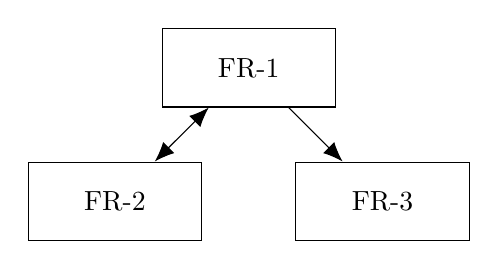
\begin{tikzpicture}[
		node distance=17mm,
		node/.style={rectangle, draw=black, minimum width=22mm, minimum height=10mm}
	]
		\node[node](fr-1){FR-1};
		\node[node](fr-2)[below of=fr-1,xshift=-17mm]{FR-2};
		\node[node](fr-3)[below of=fr-1,xshift=17mm]{FR-3};
		
		\draw[{Latex[length=2.5mm,width=2mm]}-{Latex[length=2.5mm,width=2mm]}](fr-1) -- (fr-2);
		\draw[-{Latex[length=2.5mm,width=2mm]}](fr-1) -- (fr-3);
	\end{tikzpicture}
	\caption{Functional dependency graph}
\end{figure}

\FunctionalReq
{FR-S-1}{Stability}
{Description\\Over multiple lines}
{Priority - \musthave \shouldhave \couldhave}
{No dependencies}
{Results}
{let it all crash}

\subsection{Non-functional Requirements}
\label{ssec:nf_req}

\begin{figure}[h!]
	\centering
	\begin{tikzpicture}[
		node distance=17mm,
		node/.style={rectangle, draw=black, minimum width=22mm, minimum height=10mm}
	]
		\node[node](nfr-1){NFR-1};
		\node[node](nfr-2)[below of=fr-1,xshift=-17mm]{NFR-2};
		\node[node](nfr-3)[below of=fr-1,xshift=17mm]{NFR-3};
		
		\draw[{Latex[length=2.5mm,width=2mm]}-{Latex[length=2.5mm,width=2mm]}](nfr-1) -- (nfr-2);
		\draw[-{Latex[length=2.5mm,width=2mm]}](nfr-1) -- (nfr-3);
	\end{tikzpicture}
	\caption{Non-functional dependency graph}
\end{figure}

\NonFunctionalReq
{NFR-O-1}{Modularity}
{Description\\Over multiple lines}
{No dependencies}
{Priority}
{Metrics}
{Constraints}

\NonFunctionalReqS
{NFR-S-1}{Modularity}
{Description\\Over multiple lines}
{No dependencies}
{Priority}
{Metrics}
{Constraints}
{Security}

\subsection{Risks and Issues}
\label{ssec:risks}

\subsubsection{Risk Matrix}

\RiskMatrix
{r1\\test}{r2}{r3}
{r4}{r5\\test}{r6}
{r7}{r8}{r9\\test}

\section{Project Development}
\label{sec:dev}

\subsection{Development Approach}
\label{ssec:dev_approach}

\begin{landscape}
\subsection{Project Schedule}
\label{ssec:schedule}



\centering
\begin{ganttchart}[
	x unit=0.1cm,
	y unit chart=0.5cm,
	hgrid={black!25},
	link bulge=3,
	time slot format=isodate
]{2022-10-08}{2023-4-29}
	\gantttitlecalendar{year, month=name}\\

    \ganttbar[name=req_spec]{Requirement Specification}{2022-10-21}{2022-11-10}\\
    \ganttbar[name=design_video]{Design Video Presentation}{2022-11-08}{2022-12-08}
    \ganttlink{req_spec}{design_video}
	\ganttvrule{PE 1}{2022-11-24}
	\ganttvrule{PE 2}{2022-12-08}
\end{ganttchart}
\end{landscape}

%\printbibliography

\end{document}
